% !TeX program  = xelatex
% !TeX encoding = UTF-8
% !TeX root     = 1_blockchain_types.tex
\documentclass{mirea-article}

% !TeX program  = xelatex
% !TeX encoding = UTF-8
% !TeX root     = final-qualifying-work.tex

\usepackage{hyperref}
\urlstyle{same}

\hypersetup{
    pdftoolbar=true,        % show Acrobat’s toolbar?
    pdfmenubar=true,        % show Acrobat’s menu?
    pdffitwindow=false,     % window fit to page when opened
    pdfstartview={FitH},    % fits the width of the page to the window
    pdftitle={ВКР на тему "Разработка системы токенизации дипломов на основе блокчейн-технологий для цифровой верификации и децентрализованного хранения образовательных достижений"},
    pdfauthor={М. Д. Панфилов},
    pdfsubject={Qualification Collectibles},
    pdfcreator={mxp@apteryx},
    pdfproducer={XeLaTex in VSCode},
    pdfkeywords={final qualifying work} {nft diplomas} {qualification collectibles} {educational nft}, 
    pdfnewwindow=true
}

\usepackage{comment}

\usepackage{etoolbox}

\usepackage{graphicx}

\usepackage{listings}
\usepackage{xcolor}
\lstset{basicstyle=\footnotesize, breaklines=true, numbers=left, captionpos=t, showstringspaces=false, commentstyle=\color{teal}, stringstyle=\color{red}, keywordstyle=\color{violet}}  % Настройки для всех листингов

% Введение и заключение
\newcommand{\supersection}[1]{
	\section*{#1}
	\phantomsection
	\addcontentsline{toc}{section}{#1}
}

\usepackage{caption}
\captionsetup[lstlisting]{justification=raggedright, singlelinecheck=false}

\usepackage{pdfpages}

\usepackage{microtype}

\tolerance=5000
\hbadness=9999
\emergencystretch=10pt
\hyphenpenalty=5000
\exhyphenpenalty=100

\usepackage{multirow}

\usepackage{array}
\usepackage{setspace}
\newcolumntype{x}[1]{>{\setstretch{0.8}\small\centering\arraybackslash\hspace{0pt}}m{#1}}
\newcolumntype{y}[1]{>{\centering\arraybackslash\hspace{0pt}}m{#1}}
\usepackage{longtable}

\usepackage{float}

\usepackage{listings}
\usepackage{xcolor}
\lstset{basicstyle=\footnotesize, breaklines=true, numbers=left, captionpos=t, showstringspaces=false, commentstyle=\color{teal}, stringstyle=\color{red}, keywordstyle=\color{violet}} % Настройки для всех листингов
\usepackage{caption}
\captionsetup[lstlisting]{justification=raggedright, singlelinecheck=false}

%\usepackage{color,xesearch}
%\SearchList{make-red}{\textcolor{red}{#1}}{эффективность,качество}
\usepackage{multicol}
\usepackage{ragged2e}

\newenvironment{Figure}
{\par\medskip\noindent\minipage{\linewidth}}
{\endminipage\par\medskip}

\begin{document}

\textbf{УДК 378, 004.62}

\artauthor{Панфилов Максим Дмитриевич}{студент 4 курса направления 09.03.02 <<Информационные системы и технологии>> ИКБ РТУ МИРЭА, системный архитектор ЦМАД ОАО <<ВТИ>>}{mdpanfilov@vti.ru}

\artauthor{Люцько Сергей Алексеевич}{студент 4 курса направления 09.03.02 <<Информационные системы и технологии>> ИКБ РТУ МИРЭА}{lyutsko.s.a@edu.mirea.ru}

\artauthor{Котилевец Игорь Денисович}{старший преподаватель кафедры <<Цифровые технологии обработки данных>> ИКБ РТУ МИРЭА, начальник ЦМАД ОАО <<ВТИ>>}{IDKotilevets@vti.ru}

\supersection{Классификация видов блокчейнов и их применение в различных сферах бизнеса и науки.}

Аннотация. {\itshape Целью данной статьи является выявление наиболее эффективных видов блокчейнов и механизмов достижения консенсуса в зависимости от специфики применения в финансах, здравоохранении, образовании и других ключевых областях. Особое внимание уделяется возможностям интеграции блокчейн-технологий в современные бизнес-процессы и исследовательские проекты, что позволяет наиболее полно реализовать потенциал данной технологии.}

Ключевые слова: \textit{блокчейн, публичный блокчейн, приватный блокчейн, консенсус, смарт-контракты, криптография, децентрализация, токенизация, цифровая экономика, цепочка блоков.}

\supersection{Classification of Blockchain Types and Their Applications in Various Business and Science Fields.}

Annotation. {\itshape The aim of this article is to identify the most effective types of blockchains and consensus mechanisms based on their specific applications in finance, healthcare, education, and other key areas. Special attention is given to the potential for integrating blockchain technologies into modern business processes and research projects, enabling the full realization of this technology's potential.}

Keywords: \textit{blockchain, public blockchain, private blockchain, consensus, smart contracts, cryptography, decentralization, tokenization, digital economy, chain of blocks.}

\subsection*{Введение}
\label{sec:introduction}

В условиях цифровизации экономики блокчейн-технологии приобретают особую актуальность. Это обусловлено их способностью обеспечивать прозрачность, безопасность и децентрализацию в управлении данными. Блокчейн представляет собой распределенную базу данных, где информация хранится в виде последовательно связанных блоков. Основные его особенности --- неизменяемость записей и возможность проведения операций без необходимости доверия между участниками.

Технология блокчейн имеет несколько форм, включая публичные, при-ватные и консорциумные блокчейны, каждый из которых подходит для определенных видов задач и отраслей. В этой статье осуществляется классификация основных типов блокчейнов и анализируется их применение в различных сфе-рах деятельности~\cite[с. 54 --- 61]{bib:blckgn}.

\subsection*{Виды блокчейнов и механизмы достижения консенсусов}

Блокчейн-сети можно классифицировать по нескольким критериям, включая уровень доступа к сети и механизмы достижения консенсуса (рис.~\ref{fig:types_of_blockchains}). Эти критерии определяют, как технология будет использоваться в различных сфе-рах деятельности, а также её способность обеспечивать безопасность, прозрачность и эффективность операций~\cite[с. 37 --- 75]{bib:blcktech}.


\begin{figure}[H]   
	\centering
	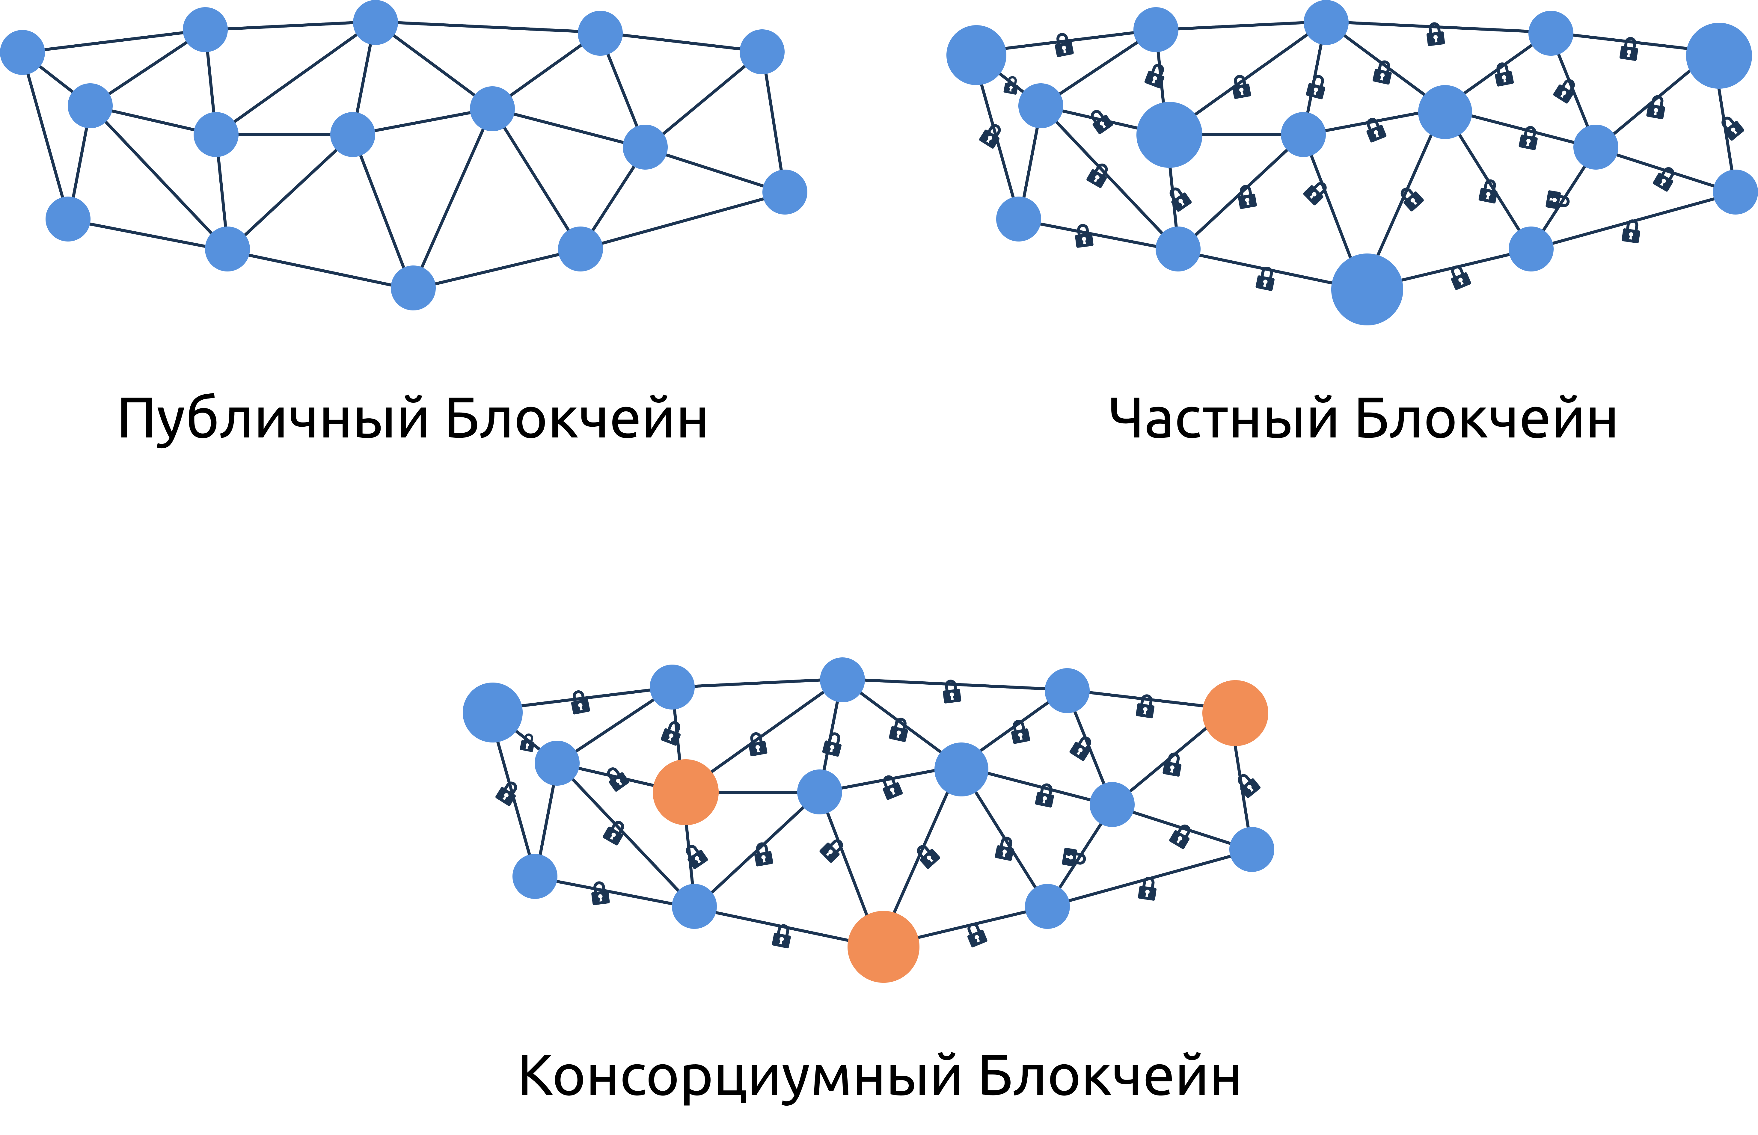
\includegraphics[width=\textwidth]{../images/types_of_blockchains.png}
	\parskip=6pt
	\caption{Классификация блокчейн-технологий по степени открытости}
	\label{fig:types_of_blockchains}
\end{figure}

Публичные блокчейны, такие, как Siberium, TON и Innochain, открыты для всех пользователей в интернете. Они позволяют любому желающему принимать участие в процессе валидации транзакций, что обеспечивает высокий уровень децентрализации и безопасности. Записи в таких блокчейнах общедоступны, что гарантирует прозрачность операций. Основной механизм достижения консенсуса в публичных блокчейнах --- это Proof of Work (PoW) или Proof of Stake (PoS), обеспечивающие защиту от мошенничества и поддержание целостности данных.

Приватные блокчейны, такие как Masterchain, Hyperledger и Corda, исполь-зуются внутри организаций или закрытых корпоративных сетях. Доступ к такому блокчейну строго регулируется и ограничен лишь участниками сети, что позволяет управлять конфиденциальностью и эффективностью обработки данных. В отличие от публичных блокчейнов, приватные системы часто используют механизмы консенсуса типа Proof of Authority (PoA) или Practical Byzantine Fault Tolerance (PBFT), которые требуют меньше ресурсов для обеспечения работы сети.

Консорциумные блокчейны представляют собой смешанный тип, объединяющий черты публичных и приватных систем. Такие блокчейны управляются группой организаций, которые совместно принимают решения по управлению и обслуживанию сети. Это позволяет сочетать высокий уровень контроля и безопасности приватных блокчейнов с некоторыми преимуществами децентрализации, характерными для публичных систем. Примеры консенсусных механизмов, используемых в таких блокчейнах, включают Multi-Signature или Delegated Proof of Stake (DPoS), которые способствуют более быстрой и эффективной обработке транзакций по сравнению с классическими публичными блокчейнами.

\subsection*{Применение в различных сферах}

В финансовом секторе блокчейн используется для улучшения прозрачности транзакций, снижения рисков мошенничества и сокращения времени обработки операций. Публичные блокчейны, такие как Bitcoin или Ethereum, позволяют создавать децентрализованные финансовые услуги (DeFi), предоставляющие пользователям доступ к финансовым услугам без посредников. Механизмы консенсуса, такие как Proof of Stake, предпочтительны из-за их энергоэффективности и быстроты в обработке транзакций по сравнению с Proof of Work~\cite{bib:blckis}.

Для логистики и управления цепочками поставок идеально подходят приватные или консорциумные блокчейны. Эти системы обеспечивают участникам рынка возможность обмениваться информацией о происхождении товаров и их перемещении в режиме реального времени, при этом сохраняя конфиденциальность коммерческой информации. Механизмы, такие как Proof of Authority или Practical Byzantine Fault Tolerance, гарантируют быструю и надежную валидацию данных при ограниченном круге участников.

В секторе энергетики блокчейн может применяться для управления данными о потреблении энергии, ее распределении и торговле углеродными кредитами. Приватные блокчейны подходят для таких задач, так как они позволяют обеспечивать безопасность данных и контролировать доступ к информации. Механизмы консенсуса, такие как PoA, обеспечивают эффективность и масштабируемость в закрытых корпоративных сетях~\cite[с. 174 --- 177]{bib:blckper}.

Блокчейн в здравоохранении может использоваться для хранения и передачи медицинских записей, обеспечивая их надежность и доступность при соблюдении требований конфиденциальности. Консорциумные блокчейны с механизмами консенсуса типа Multi-Signature или PBFT предлагают баланс между контролем доступа и децентрализацией, что критически важно для соблюдения законодательства о защите данных.

В образовании и науке блокчейн может применяться для цифровой аттестации квалификаций, публикации и проверки научных работ. Публичные блокчейны с механизмом консенсуса PoS или DPoS позволяют обеспечить неприкосновенность и проверяемость академических достижений, а также способствуют улучшению коллаборативности в научных исследованиях.

\subsection*{Вывод}

Потенциал блокчейн-технологий в современной экономике трудно переоценить. Их способность адаптироваться к различным условиям и требованиям делает их незаменимым инструментом в руках тех, кто стремится к инновациям и эффективности. Ожидается, что дальнейшее развитие и интеграция блокчейн-технологий принесет новые возможности для улучшения бизнес-процессов, укрепления безопасности данных и углубления цифровой трансформации во всех сферах жизнедеятельности.


\begin{thebibliography}{99\kern\bibindent}
    \bibitem{bib:blckgn} Годин В.В., Терехова А.Е. Блокчейн: философия, технология, приложения и риски. // Журнал <<Вестник университета>> --- 2019. --- №9.

    \bibitem{bib:blcktech} Носиров З.А., Фомичев В.М. Анализ блокчейн-технологии: основы архитектуры, примеры использования, перспективы развития, проблемы и недостатки // Журнал <<Системы управления, связи и безопасности>> --- 2021. --- №2.

    \bibitem{bib:blckis} Федотова В.В., Емельянов Б.Г., Типнер Л.М. Понятие блокчейн и возможности его использования. // Журнал <<European science>> --- 2018.

    \bibitem{bib:blckper} Бердышев А.В., Соловьев А.Н. Перспективы развития российского электроэнергетического комплекса на основе технологии блокчейн. // Журнал <<Финансовые рынки и банки>> --- 2023. --- №6.
\end{thebibliography}

\end{document}